\documentclass{homework}
% \usepackage{lua-visual-debug}
\usepackage{graphicx}
\usepackage{amsmath, amssymb, amsfonts}
\usepackage{enumitem}
\usepackage{ulem}
\usepackage{tikz}
\usepackage[a4paper, total={6in, 8.8in}]{geometry}

\title{Practice \#5}
\subject{CS341 Introduction to Computer Networks}
\studentid{20170058}
\name{Keonwoo Kim}
\date{\today}

\begin{document}
\maketitle

\parindent=0pt


\solution{
    \vspace*{-1.3em}
    \begin{enumerate}[label={1.\arabic*.}, topsep=-2em]
        \item \hfill\\
        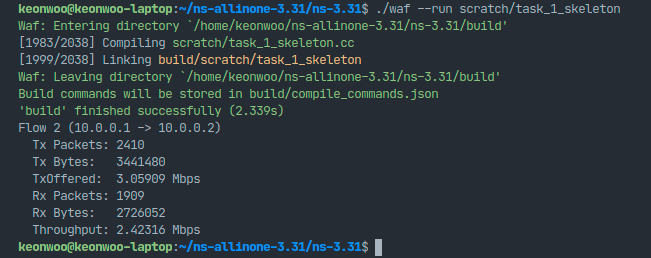
\includegraphics[width=\linewidth]{task1-1}
        \item The blue line in the figure below represents the result of the simulation using \texttt{WIFI\_PHY\_} \texttt{STANDARD\_80211g}:\\
        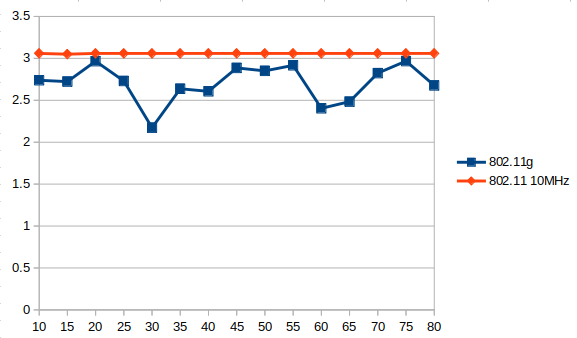
\includegraphics[width=\linewidth]{task1-2}
        Using 2.4 GHz networks, the throughput varies over the distance between A and B.
        \item[1.3.1.] Using \texttt{WIFI\_PHY\_STANDARD\_80211\_10MHZ}, there are (almost) no decrease in the throughput, while \texttt{WIFI\_PHY\_STANDARD\_80211g} shows a decrease in the throughput. Thus, 5 GHz communication is more robust to interferences.
        \item[1.3.2.] \texttt{WIFI\_PHY\_STANDARD\_80211\_10MHZ} is for 5 GHz networking, while \texttt{WIFI\_PHY\_STANDARD\_80211g} is for 2.4 GHz networking.
        \item[1.4.] When the position of Node C is moved to $(-1000000, 0, 0)$, far enough from A and B, the throughput is close to 3.05909 Mbps, which is the maximum rate. So, we can guess that the role of Node C is to give an interference to the communication.
    \end{enumerate}
    \vspace*{3.3em}
}



\solution{
    \vspace*{-1.3em}
    \begin{enumerate}[label={2.\arabic*.}, topsep=-2em]
        \item[2.5.] The right one is for 2.5.1. and the left one is for 2.5.2.
         
        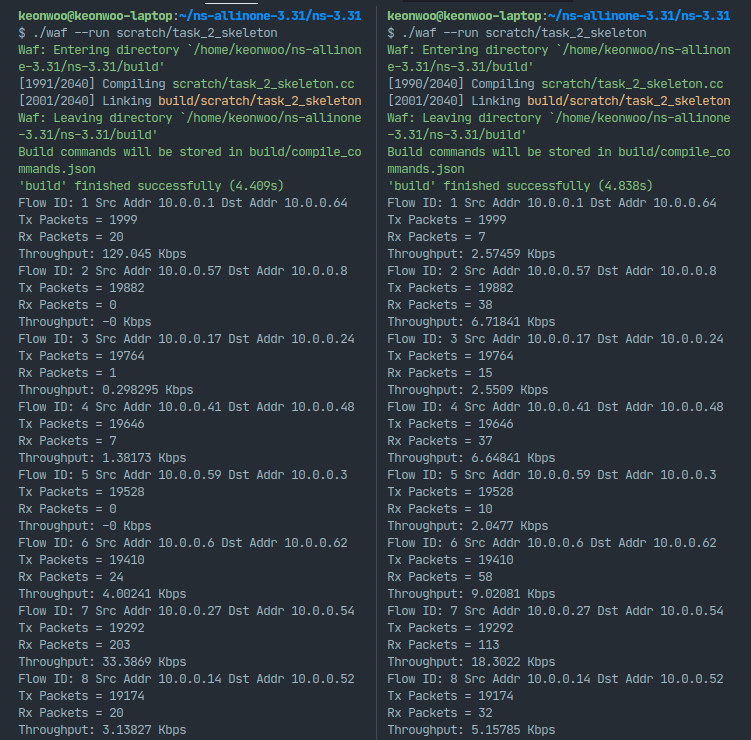
\includegraphics[width=\linewidth]{task2-1}
        \item[2.5.3.] In general, the experiment with RTS/CTS enabled shows higher throughputs than one with RTS/CTS disabled. Since RTS/CTS is used to reduce frame collisions due to hidden node problems, it will reduce frame collisions and the throughput will increase.
    \end{enumerate}
    \vspace*{3.3em}
}

\newpage

\solution{
    \hfill\\ 
    
\includegraphics[width=\linewidth]{task3-1}
}

\end{document}